\chapter{Introduction}
\index{Introduction@\emph{Introduction}}
%\index{Making Tables and Including Figures@\emph{Making Tables
%	and Including Figures}}%

GPUs cater to highly parallel and regular computation patterns. While GPUs provide hardware specifically tailored for parallel problems, good GPU performance relies on programs exhibiting behavior that can be partitioned into separate threads of computation. Warps are what we call a collection of threads that run in lock-step, and all threads within a warp should run similar code and access relatively nearby data in memory. Data-divergence occurs when these warps overload lower-level memory systems by accessing many different pieces of data simultaneously. Our goal in this paper, with both Hawkeye and precleaning, is to limit and offset the negative performance impacts of both data-divergence and poorly optimized access patterns.

Computer architects have been using caches and smart cache replacement policies to hide the latency of predictable memory operations for decades \cite{deadblock,lruperf,cache_burst,dip,eva,rrip} [can cite quite a few here]. Caches decide to hold on to heavily reused memory lines to hide latency of repeated memory accesses. LRU is the baseline replacement policy for most caches as it is easy to reason about and performs well considering its relative simplicity. LRU can’t handle complex access patterns like streaming and does not store any information on lines previously evicted from the cache. Thus when GPU code starts to exhibit data-divergent behaviour, a cache that can handle irregular or complex access patterns can filter out some of the requests that would otherwise overload our main memory. By providing a proven and theoretically sound approach to cache replacement, we hope to improve performance on GPU programs that would previously see no benefit from the cache due to said programs’ abnormal access patterns.

Our goal is to evaluate and use Hawkeye \cite{hawkeye}, a CPU cache replacement policy that excels at capturing complex data reuse patterns. Hawkeye prefers to evict lines similar to other lower performing lines in the OPTGen algorithm, an online approximation of Belady’s optimal cache replacement policy. We evaluate features, such as warp ID and PC, that we believe work well in a GPU context. We also explore the application of Hawkeye in both the L1 and L2 caches.

We believe we can improve performance of our caches beyond just changing replacement policies. Write-through and write-back caches are the two main ways that modern caches handle mutable data within the cache. Write-through caches immediately write modified data back to their backing store (such as a lower level cache or DRAM). On the other hand, write-back caches delay committing writes to their backing store until the associated line is evicted. This delay in commiting writes is possible because non-atomic writes are off the critical path, meaning the processor will never need to stall for a non-atomic write. Write-back caches tend to be more efficient than write-through caches as write-through caches require an access to lower level memory for every single write. While the strategy of writing back at the last possible moment might be the most convenient, it is not necessarily the most optimal time for data to be written back to lower level memory. Writing back at the time of eviction can be especially problematic in GPUs when unoptimized parallel code causes many simultaneous evictions. The key takeaway is that, rather than a binary choice of write-through and write-back, we actually have a full spectrum of choices to choose from when cleaning dirty cache lines. Please refer to Figure \ref{f:bandwidth_optimal} for a visualization of this spectrum.

\begin{figure}[htb]
\begin{center}
\ 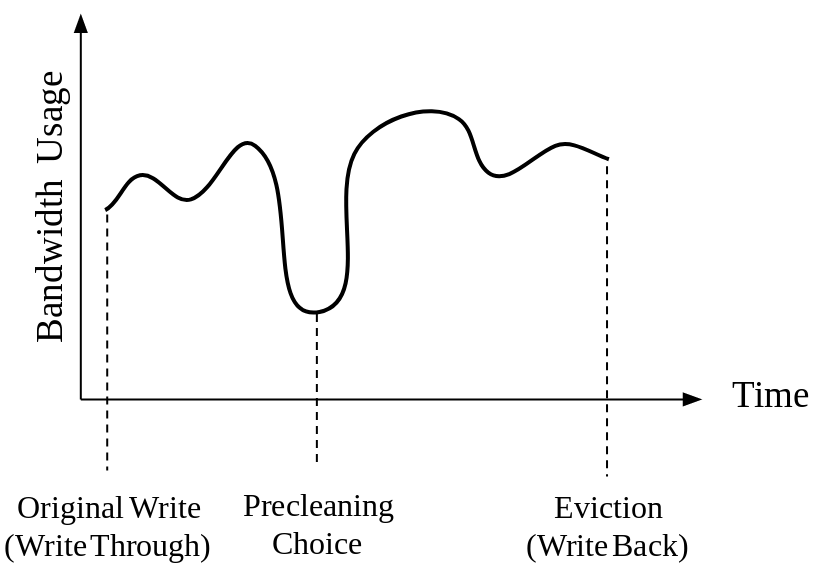
\psfig{file=figs/bandwidth_optimal.png,width=\textwidth}
\caption{Example of cache cleaning choices, showing potential improvement for bandwidth usage.}
\label{f:bandwidth_optimal}
\end{center}
\end{figure}
\index{commands!environments!figure}%

To further improve GPU memory system performance, we would like to use previous data and current memory bandwidth usage levels to know when it’s best to write back modified cache lines. We believe that GPUs are a good fit for this problem due to the parallel nature of the hardware. Making accesses to memory across many cores increases the chances of multiple write-backs being triggered around the same time. GPUs are very reliant on having adequate bandwidth available to hide latency across all cores. When bandwidth saturates, our code will effectively start to serialize, causing us to lose the performance benefits of our parallel architecture. A perfect solution would evenly spread out all write-back traffic, preventing bandwidth spikes that could stall our GPU cores.
